\documentclass{article}
\usepackage[a4paper, width=170mm, top=20mm, bottom=20mm]{geometry}
\usepackage{hyperref}
\usepackage{amsmath}
\usepackage{nopageno}
\usepackage{xcolor}
\usepackage{adjustbox}
\newcommand\tab[1][0.5cm]{\hspace*{#1}}
\usepackage{mdframed}
\newmdenv[linecolor=white,backgroundcolor=blue!10]{myframe}
\usepackage{graphicx}
\usepackage{subcaption}
\usepackage{amsmath}
\usepackage{bm}
\usepackage{lipsum}
\usepackage[shortlabels]{enumitem}
\usepackage{fancyhdr}
\pagestyle{fancy}
\renewcommand{\headrulewidth}{0pt}
\fancyhead{}
\fancyfoot{}
\fancyfoot[C]{\thepage}

% Set greek language
%\usepackage[english,greek]{babel}
\usepackage[utf8]{inputenc}
%\newcommand{\en}[1]{\foreignlanguage{english}{#1}}
%\usepackage{kerkis} 
%\usepackage{abc}

% Hyperref
\usepackage{hyperref}
\hypersetup{
	colorlinks=true,
	linkcolor=black,
	filecolor=black,      
	urlcolor=blue,
}

% Tables
\usepackage{tabu}
\usepackage{tabularx}
\newcolumntype{L}[1]{>{\raggedright\let\newline\\\arraybackslash\hspace{0pt}}m{#1}}
\newcolumntype{C}[1]{>{\centering\let\newline\\\arraybackslash\hspace{0pt}}m{#1}}
\newcolumntype{R}[1]{>{\raggedleft\let\newline\\\arraybackslash\hspace{0pt}}m{#1}}

\begin{document}


\noindent
\begin{huge}
\hspace{-3.0mm}\textbf{OpenFOAM Tutorials}
\end{huge}

\setcounter{section}{2}
\section{Zones}
	
\begin{enumerate}[3.1]
	\item In this step we will model the heat transfer between two separate regions, the air region, and a solid plate. In both regions the Laplace equation must be solved. In the following figure the problem parameters, the geometry, the initial and the boundary conditions can be seen. The previously created {\tt laplaceFoam} solver can be modified to the needs of this problem. The new solver will be named {\tt laplaceMultiRegionFoam}. The parameters of the problem are $L=2~m$, $H=1~m$, $T_L=350~K$ and $T_R=300~K$.
	
	\begin{center}
		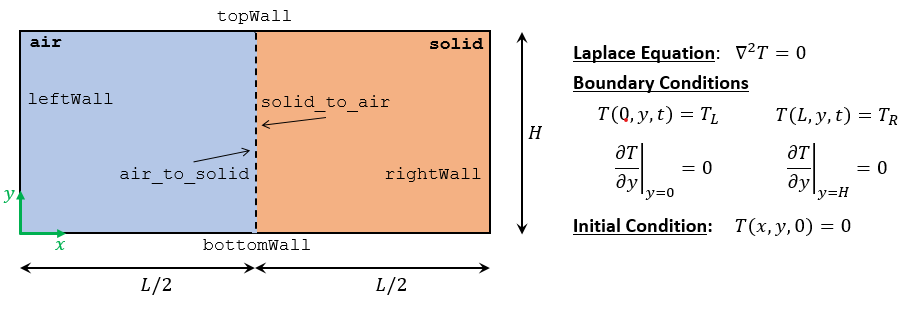
\includegraphics[width=0.8\textwidth]{laplace_airSolid.png}
	\end{center}

	To solve the Laplace equation two regions, two zones must be created (there are two ways to achieve that), one for each region. The first region will be named solid and the other one air, and in each region two separate Laplace equations will be solved, in two different meshes. In the interface between those two regions, the boundary condition must be suitable defined so that the two solutions of the temperature (one for the solid and one for the air) are coupled. More in particular, the value and the normal derivative of the temperature in the interface must be equal
	
	$$ 
	T_{air} = T_{solid} 
	$$
	$$	
	k_{air} \dfrac{\partial T}{\partial n} \Bigg|_{air} = k_{solid} \dfrac{\partial T}{\partial n} \Bigg|_{solid} 
	$$
	
	where $k$ is the thermal conductivity of each region. 
	
	In the following steps, two different ways of defining multiple regions will be described, which can be found in the {\tt case1} and {\tt case2} folders respectively.
	
	\item The first method of creating multiple regions is by using the {\tt topoSet} tool, which can be found in {\tt ./tutorials/zones/case1/} directory. In the {\tt blockMeshDict} a rectangular mesh block is defined, in the size of both the air and solid regions. In the {\tt topoSetDict} the user can choose with the {\tt boxToCell} command which cells of the domain will belong to the solid region, while the rest will be the air. In this example, the name of the zone is 'solid', which contains one {\tt cellSet} called 'solidSet'. The {\tt boxToCell} can be larger than the domain, as it recognizes the cell centers that belong inside the box.
	
	So after running the {\tt blockMesh} command to define the geometry, the {\tt topoSet} command defines the zones.
	
	The next step is to split the domain into all the defined regions, two in this case, one region will be the solid plate, and the remaining cells will be the air. The command is
	
	{\tt
	\tab \$ splitMeshRegions -cellZones -overwrite
	}

	Before running the {\tt splitMeshRegions} command, the directory {\tt ./0/} must be renamed (for example ./0.org/) in order to avoid any boundary conditions errors. After the successful execution of the command, the directory can be renamed in its original name.
	
	After running these commands, two regions will be created, the 'solid' region, and a region called 'region1', which is the remaining cells. The default region that is used by OpenFoam, that corresponds to the {\tt polyMesh} is called 'region0', so some changes must be made in the {\tt ./constant/} and {\tt ./system/} directories. In the {\tt ./constant/} directory three folders exist:
	
	\begin{itemize}
		\item[--] the {\tt polyMesh} folder that corresponds to the original mesh before the command {\tt splitMeshRegions}
		
		\item[--] the {\tt solid} folder that corresponds to the solid region, as defined after the {\tt splitMeshRegions} command
		
		\item[--] the {\tt region1} folder which contains the remaining cells, which correspond to the air.
	\end{itemize}

	As the original {\tt polyMesh} folder is not necessary anymore, it must be removed, and in its place the {\tt ./constant/region1/polyMesh/} directory must be placed. Moreover various changes must me made in the {\tt ./constant/polyMesh/boundary} and {\tt ./constant/solid/polyMesh/boundary} files, so that the 'region1' entries are replaced with 'region0'.
	
	As for the boundary conditions, two new boundaries will be created after the {\tt splitMeshRegions} command, the {\tt solid\_to\_region0} and the {\tt region0\_to\_solid} boundaries, which correspond to the solid region and air region (region0) respectively. The interface boundary condition is the following
	
	\begin{myframe}
	{\tt 
    	region0\_to\_solid\\
		\{\\
		\tab type~~~~~~~~~~compressible::turbulentTemperatureCoupledBaffleMixed;\\
		\tab value~~~~~~~~~\$internalField;\\
		\tab Tnbr~~~~~~~~~~Tsolid;\\
		\tab kappaMethod~~~lookup;\\
		\tab kappa~~~~~~~~~kappaA;\\
		\}
	}
	\end{myframe}
	
	where {\tt Tsolid} is the temperature field in the solid region, and {\tt kappaA} is a {\tt scalarField} whose value is equal to the thermal conductivity of the air in every cell. In a similar way the {\tt solid\_to\_region0} boundary condition can be created.
	
	\item As for the solver, it is necessary to define two separate meshes, one is the default {\tt mesh} and one is the {\tt meshS}, defined in the {\tt createMeshS.H} file. This file must be included in the main program. In the {\tt createFields.H} and {\tt createFieldsSolid.H} all the necessary fields and variables are defined. Each field is assigned to either {\tt mesh} or {\tt meshS}, according to whether the variable corresponds to the solid region or the air region. As it can be seen in the main program, there are two different laplace equations being solved, one for the air region and one for the solid region.
	
	Moreover, in order for the {\tt compressible::turbulentTemperatureCoupledBaffleMixed} boundary condition to work, extra OpenFOAM libraries must be defined in the {\tt ./Make/options} file.
	
	\item Now, after studying the structure of the case and solver, you can run the simulation. Before doing that, there are some necessary actions that must be taken. First of all, to define the appropriate schemes and solution algorithms in the {\tt fvSchemes} and {\tt fvSolution} files. Note that in the {\tt ./system/} directory the schemes and solution algorithms of the region0 must me defined, and in the {\tt ./system/solid} directory the schemes and solution algorithms of the solid region. For convenience, you can define in a single {\tt fvSchemes} and {\tt fvSolution} file all necessary entries for both regions, and copy them in both the {\tt ./system/} and {\tt ./system/solid} directories. 
	
	Next, the flow and fluid parameters must be defined in the {\tt physicalProperties} and {\tt regionProperties} files. Lastly, you must be sure that the correct boundary conditions are implemented in the {\tt ./0/} and {\tt ./0/solid} directories.
	
	Due to the complexity and amount of all the above commands, it is convenient to create a single terminal executable bash script that contains all the previous commands that built the case, and run only this script instead. As it can be seen in the example case, there are three bash scripts available:
	
	\begin{itemize}
		\item[--] {\tt Allmesh}: This script runs the {\tt blockMesh}, {topoSet} and {\tt splitMeshRegions} commands. Also it converts the region1 into the polyMesh, and it copies the {\tt fvSchemes} and {\tt fvSolution} files in all region folders. Also it temporarily renames the {\tt ./0/} directory, in order to avoid any errors. According to the application, the user can add or remove any other commands that are necessary to successfully built the case. It also created a {\tt .log} file with the mesh size and parameters, using the {\tt checkMesh} command.
		
		\item[--] {\tt Allclean}: This script cleans and deletes all the created files by the {\tt Allmesh}.
		
		\item[--] {\tt run}: This file runs the declared solver in the {\tt controlDict} file.
	\end{itemize}
	
	
	To run any of the bash scripts, just run the command (e.g. for the {\tt Allmesh} script)
	
	{\tt 
	\tab \$ ./Allmesh	
	}
	
	\textbf{Tip}: Make sure that your system recognizes the bash scripts as executables.
	
	
	\item The second method of creating multiple regions, is to explicitly declare them from the {\tt blockMeshDict} file, instead of using the {\tt topoSet} utility. You can create multiple blocks, and declare that the particular block is a part of the desired zone. This not only simplifies the constructing of the case by having to modify less files whenever one wishes to change the geometry, but also has quicker and less prone to build errors. Moreover, the way that the {\tt topoSet} tool works is that it chooses which cells will be part of a specific zone, by whether the coordinates of their centers are within the desired region (box, cylinder, circle, etc.). This means that according to the size of the cells, the boundaries of the region might be slightly different, ehich may result to substantial errors.
	
	The only drawback with this method is that the block as a whole must be a part of the zone, and not a part of it, like with the {\tt topoSet} tool. This sometimes might result in complicating the construction of the {\tt blockMeshDict} file. 
	
	The {\tt ./tutorials/zones/case2/} directory contains the test case, along with the corresponding solver. It is of similar logic, with the difference that here there is no {\tt region0} or {\tt polyMesh} folder, but there are two blocks, one for the air region and one for the solid region. The declaration of the zone can be seen below in the {\tt blockMeshDict} file.
	
	
	\begin{myframe}
	{\tt 
		
	vertices\\
	(\\
	\tab (0 0 0)~~~~~// point 0\\
	\tab (1 0 0)~~~~~// point 1\\
	\tab (1 1 0)~~~~~// point 2\\
	\tab (0 1 0)~~~~~// point 3\\
	\tab (0 0 0.1)~~~// point 4\\
	\tab (1 0 0.1)~~~// point 5\\
	\tab (1 1 0.1)~~~// point 6\\
	\tab (0 1 0.1)~~~// point 7\\
	\tab (2 0 0)~~~~~// point 8\\
	\tab (2 1 0)~~~~~// point 9\\
	\tab (2 0 0.1)~~~// point 10\\
	\tab (2 1 0.1)~~~// point 11\\
	);\\
	\\
	blocks\\
	(\\
	\tab hex (0 1 2  3  4  5  6  7) air (20 20 1) simpleGrading (1 1 1)\\
	\tab hex (1 8 9 2 5 10 11 6) solid (20 20 1) simpleGrading (1 1 1)\\
	);
	}
\end{myframe}
	
	After executing the {\tt splitMeshRegions} command
	
	{\tt
	\tab \$ splitMeshRegions -cellZones -overwrite
	}
	
	the desired regions will have been created. If we wanted the {\tt region0} to exist, then can just delete the 'air' word from the block definition.
	
	Now that there is no {\tt region0} or {\tt polyMesh}, the rest of the files of the case, must be modified accordingly. Note that this way there is no need to temporarily rename the {\tt ./0/} directory.
	
	The solver must be modified as well, because we need to define two extra meshes, {\tt meshA} for the air region, and {\tt meshS} for the solid region. The corresponding {\tt createMesA.H} and {\tt createMesS.H} must be included in the main program as well.
	
	\item Run the simulations, and verify that the two methods, {\tt case1} and {\tt case2} produce identical results.
	
	
\end{enumerate}


%	
%	Η οριακή συνθήκη που χρησιμοποιείται είναι η:
%	
%	\tab \en{\tt compressible::turbulentTemperatureCoupledBaffleMixed}
%
%	και μπορεί να βρεθεί ο τρόπος χρήσης της, όπως και ο τρόπος δημιουργίας \en{regions} με το \en{\tt topoSet} (αρχείο \en{\tt topoSetDict}), από τα \en{tutorial cases} του λύτη \en{\tt chtMultiRegionFoam}, που βρίσκεται στην κατηγορία \en{heat transfer}. 
%	
%	Επιπλέον, θα πρέπει να δημιουργηθούν στον \en{solver} δύο διαφορετικά πλέγματα, όπου στο ένα (\en{meshA}) θα λυθεί η εξίσωση \en{Poisson} για τον αέρα και στο άλλο (\en{meshS}) θα λυθεί η εξίσωση \en{Laplace} στο στερεό. Αυτό συνεπάγεται, πως θα υπάρχουν δύο διαφορετικές μεταβλητές (\en{\tt scalarFields}) στο αρχείο \en{\tt createFields.h}, μία για την θερμοκρασία στον αέρα \en{\tt Tair} και μία για την θερμοκρασία στο στερεό \en{\tt Tsolid}. Αντίστοιχα, όπως αναφέρθηκε προηγουμένως, θα πρέπει να υπάρχουν δύο διαφορετικές εξισώσεις στο αρχείο \en{\tt laplaceFoam.c}, η \en{Poisson} για την \en{\tt Tair} στο \en{meshA}, και η \en{Laplace} για την \en{\tt Tsolid} στο \en{meshS}.
%	
%	Θα πρέπει να υπάρχουν, αντίστοιχα και στο \en{case} δύο διαφορετικά αρχεία για τις συνοριακές συνθήκες και να τοποθετηθούν στους φακέλους που θα δημιουργηθούν μετά την χρήση του \en{\tt topoSet}, στις διαδρομές \en{\tt ./0/air} και \en{\tt ./0/solid} . Σε κάθε αρχείο συνοριακής συνθήκης θα πρέπει να προστεθεί και η συνθήκη για την διεπιφάνεια. Ο ακριβής τίτλος του συνόρου των διεπιφανειών (μία για κάθε \en{region}) δημιουργείται αυτόματα από την εντολή \en{\tt topoSet} και μπορεί να βρεθεί στις διαδρομές \en{\tt ./constant/air} και \en{\tt ./constant/solid}. Τέλος, πρέπει να σημειωθεί, πως για την σωστή λειτουργία της συνοριακής συνθήκης \en{\tt BaffleMixed} θα πρέπει να δημιουργηθούν δυο \en{scalar} μεταβλητές π.χ. \en{kappaA} και \en{kappaS} οι οποίες θα έχουν την τιμή των σταθερών $k_{air}$ και $k_{solid}$ σε ολόκληρο το \en{region} που αντιστοιχεί σε κάθε μεταβλητή.
%	
%	Παράδειγμα της συνοριακής συνθήκης για την μεταβλητή \en{\tt Tair} φαίνεται παρακάτω.
%	
%	\hspace{0.4cm}
%	\begin{minipage}{0.92\textwidth}
%	\begin{myframe}
%	\en{\tt %
%    air\_to\_solid\\%
%		\{\\%
%		\tab	type  ~~~~~~~~~~          compressible::turbulentTemperatureCoupledBaffleMixed;\\%
%		\tab	value  ~~~~~~~~~         \$internalField;\\%
%		\tab	Tnbr   ~~~~~~~~~~         Tsolid;\\%
%		\tab	kappaMethod ~~~    lookup;\\%
%		\tab	kappa    ~~~~~~~~~       kappaA;\\%
%		\}\\%
%	}
%	\end{myframe}
%	\end{minipage}
%	
%	
%	
%	
%	
%	
%	
%
%	
%	
%\end{enumerate}










\end{document}